\documentclass[11pt]{article}
% Shared preamble for the research-note series.
% Create note-specific content in the per-note directory; keep common macros here.
\usepackage[margin=1in]{geometry}
\usepackage[T1]{fontenc}
\usepackage[utf8]{inputenc}
\usepackage{amsmath,amssymb}
\usepackage{booktabs,longtable,array}
\usepackage{graphicx}
\usepackage{float}
\usepackage{enumitem}
\usepackage{xcolor}
\usepackage{hyperref}
\usepackage{caption}
\usepackage{titlesec}
\hypersetup{colorlinks=true, linkcolor=blue!60!black, urlcolor=blue!60!black, citecolor=blue!60!black}
\setlist[itemize]{leftmargin=1.25em, itemsep=0.2em, topsep=0.3em}
\setlist[enumerate]{leftmargin=1.4em, itemsep=0.2em, topsep=0.3em}
\setlength{\parindent}{0pt}
\setlength{\parskip}{0.6em}
\newcommand{\statusbox}[2]{%
  \noindent\fcolorbox{black}{gray!10}{%
    \parbox{\dimexpr\linewidth-2\fboxsep-2\fboxrule\relax}{%
      \textbf{Status:} #1\\#2
    }%
  }
}

% Shared notation helpers for the research-note series.
\newcommand{\Jlin}{J}
\newcommand{\Jphys}{J_{\mathrm{phys}}}
\newcommand{\Jsurf}{J_{\mathrm{surf}}}
\newcommand{\JdB}{J_{\mathrm{dB}}}
\newcommand{\phiopt}{\phi_{\mathrm{opt}}}
\newcommand{\sigmathreedb}{\sigma_{3\mathrm{dB}}}
\newcommand{\Nt}{N_t}
\newcommand{\Nphi}{N_{\phi}}
\newcommand{\Lfiber}{L}
\newcommand{\Pcont}{P}
\newcommand{\band}{\mathcal{B}_{\mathrm{Raman}}}
\newcommand{\todoitem}[1]{\textcolor{red!70!black}{\textbf{TODO:} #1}}


\title{Warm-Start Re-Optimization for Long-Fiber Raman Suppression}
\author{Fiber Raman Suppression Project}
\date{Evidence snapshot: 2026-04-28}

\begin{document}
\maketitle

\begin{abstract}
Long fibers are expensive to optimize because each objective and gradient
evaluation requires a long propagation solve.  This note documents a practical
shortcut: optimize a phase mask on a cheaper short target, transfer that mask
to a long-fiber grid, and then re-optimize the long target from the transferred
mask instead of starting from a flat phase.  In the current single-mode SMF
evidence, a short-fiber mask already gives roughly $-51.5$ dB Raman-band
fraction when evaluated at $100$ m, and long-target re-optimization improves it
to the mid-$-50$ dB range.  The result is important as a strategy, but it is not
yet a converged claim about the global optimum at $100$ m.
\end{abstract}

\section*{Claim Status}
\statusbox{provisional but important}{The warm-start/re-optimization strategy is supported by real 50--100 m runs and standard images.  The long-fiber optimum is still not fully converged, so this note should be read as a research strategy note rather than a final performance benchmark.}

\section{Question}

The practical question is simple:

\begin{quote}
Can we make long-fiber optimization cheaper by first learning a useful phase
mask on a short fiber, then using that mask as the initial guess for the long
fiber?
\end{quote}

This is different from physically re-shaping the pulse inside the fiber.  The
current evidence is about a \emph{computational warm start}: the same input
phase is optimized again against a longer target length.  A physical segmented
experiment, where a pulse is reshaped after some propagation distance, would be
a different hardware problem.

\begin{figure}[H]
\centering
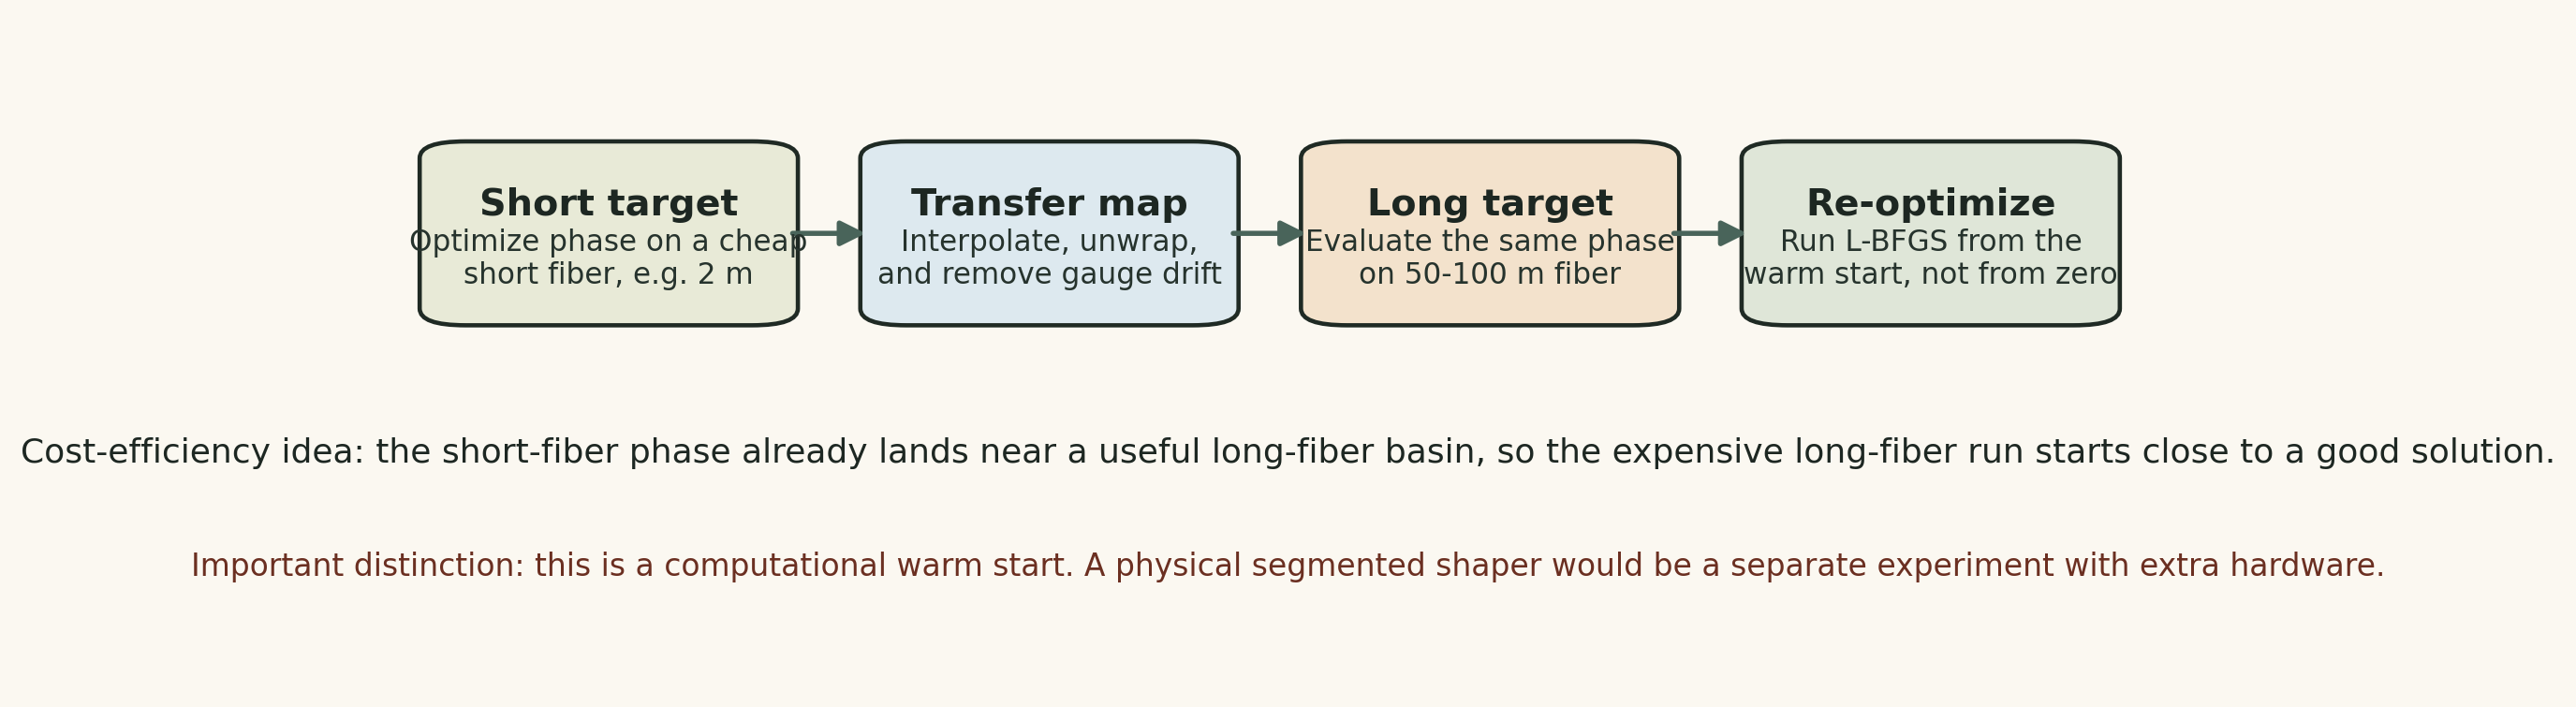
\includegraphics[width=0.96\linewidth]{figures/warm_start_reoptimization_workflow.png}
\caption{Warm-start re-optimization workflow.  The short target gives a cheap
first mask; the long target then uses that mask as an initial condition instead
of beginning from zero phase.}
\end{figure}

\section{Cost Function and Propagation Setup}

The scalar cost is the same Raman-band energy fraction used in the rest of the
single-mode optimization work:
\begin{equation}
J(\phi;L)=
\frac{\displaystyle\sum_{k\in \band} |\hat u_k(L;\phi)|^2}
{\displaystyle\sum_k |\hat u_k(L;\phi)|^2}.
\label{eq:raman-fraction}
\end{equation}
Most reported values use
\begin{equation}
J_{\mathrm{dB}}(\phi;L)=10\log_{10}J(\phi;L).
\label{eq:db-cost}
\end{equation}
More negative values mean less energy in the Raman-shifted band.

The shaped input spectrum is
\begin{equation}
\hat u_k(0;\phi)=\hat u_{0,k}\exp(i\phi_k),
\label{eq:input-phase}
\end{equation}
where the amplitude $\hat u_{0,k}$ is fixed and only the spectral phase is
optimized.  Long-fiber propagation then evaluates the generalized nonlinear
Schr\"odinger model with dispersion and the delayed Raman response.  The
propagation details are inherited from the main single-mode model; this note is
only changing the \emph{initialization strategy} for the optimizer.

\paragraph{TL;DR.}
The optimizer is still minimizing the same Raman fraction.  The only trick is
that the long run starts from a phase mask that was already useful on a shorter
fiber, instead of asking L-BFGS to discover the whole structure from a flat
phase.

\section{Transfer Map}

Let $\phi_s$ be the phase optimized on a short fiber length $L_s$, and let
$\omega^{(s)}$ and $\omega^{(\ell)}$ be the short and long frequency grids.  The
long-fiber initial phase is a transferred version of the short phase:
\begin{equation}
\phi_{\mathrm{init},j}^{(\ell)}
= \mathcal I\!\left[\operatorname{unwrap}(\phi_s)\right]\!
\left(\omega^{(\ell)}_j\right),
\label{eq:interpolation}
\end{equation}
where $\mathcal I$ is interpolation on physical angular frequency.  Frequencies
outside the short-grid support are set conservatively rather than extrapolating
large artificial phase structure.

After interpolation, the phase may be gauge-centered because a constant phase
does not change the spectral intensity objective:
\begin{equation}
\phi_{\mathrm{init}}^{(\ell)}
\leftarrow
\phi_{\mathrm{init}}^{(\ell)}
-\frac{1}{N}\mathbf 1\mathbf 1^T\phi_{\mathrm{init}}^{(\ell)}.
\label{eq:gauge}
\end{equation}
The long optimization then solves
\begin{equation}
\phi_{\ell}^{*}\approx
\arg\min_{\phi} J_{\mathrm{dB}}(\phi;L_{\ell}),
\qquad
\phi^{(0)}=\phi_{\mathrm{init}}^{(\ell)}.
\label{eq:warm-reopt}
\end{equation}

\paragraph{Intuition Check.}
In linear algebra terms, this is not a new objective.  It is a better starting
vector.  The short-fiber solution gives L-BFGS a point that already has useful
destructive-interference structure, so the expensive long-fiber search spends
more time refining and less time discovering the basic mask shape.

\section{Experimental Method}

The current long-fiber evidence uses a single-mode SMF-style setup with
$L=50$ m and $L=100$ m targets.  The $100$ m configuration used a large time
window and grid to avoid edge artifacts: $\Nt=32768$ and a $160$ ps time
window.  The primary warm start came from a short-fiber optimized mask at
$L_s=2$ m.

\begin{table}[H]
\centering
\small
\begin{tabular}{>{\raggedright\arraybackslash}p{0.24\linewidth}>{\raggedright\arraybackslash}p{0.66\linewidth}}
\toprule
Step & What was done \\
\midrule
Short optimization & Obtain a phase mask on the cheap short target. \\
Transfer & Interpolate the unwrapped short mask onto the long-fiber frequency grid. \\
Warm-start evaluation & Propagate the transferred mask at the long length without updating it. \\
Re-optimization & Run L-BFGS on the long target, initialized from the transferred mask. \\
Diagnostics & Save the standard image set, energy/edge checks, final cost, gradient norm, and convergence flag. \\
\bottomrule
\end{tabular}
\caption{Minimal experimental protocol for the warm-start re-optimization lane.}
\label{tab:protocol}
\end{table}

\section{Representative Results}

\begin{table}[H]
\centering
\small
\begin{tabular}{>{\raggedright\arraybackslash}p{0.42\linewidth}cc>{\raggedright\arraybackslash}p{0.18\linewidth}}
\toprule
Configuration & Length & Raman fraction & Status \\
\midrule
No shaping / flat phase & $100$ m & $-0.20$ dB & control \\
Transferred short-fiber mask, no re-optimization & $100$ m & $-51.50$ dB & warm-start only \\
Long-fiber re-optimization from warm start & $100$ m & $-54.77$ dB & archived run, not converged \\
Long-fiber re-optimization from warm start & $100$ m & $-55.92$ dB & later rerun, not converged \\
\midrule
No shaping / flat phase & $50$ m & $-1.91$ dB & control \\
Transferred short-fiber mask, no re-optimization & $50$ m & $-51.92$ dB & warm-start only \\
Long-fiber re-optimization from warm start & $50$ m & $-60.74$ dB & short re-opt run \\
\bottomrule
\end{tabular}
\caption{Current evidence for long-fiber warm starts.  The main supported claim
is not that the long-fiber optimum is finished; it is that the short-fiber mask
lands extremely close to a useful long-fiber basin.}
\label{tab:results}
\end{table}

At $100$ m, the warm start alone gives about $51$ dB improvement over the flat
phase control.  Re-optimization gives another $3$--$4$ dB in the available
runs.  At $50$ m, re-optimization gave a larger extra improvement, about
$8.8$ dB beyond the transferred mask.  This supports the view that warm starts
are valuable, but the amount of extra gain depends strongly on length and on
whether the long optimization has actually converged.

\subsection*{Provenance Check}

The numbers and images in this note are based on saved long-fiber artifacts and
standard image sets.  The strongest table entries are the $100$ m no-shaping
control, the transferred-mask evaluation, and the warm-started re-optimization
reruns.  The important caveat is convergence: the available $100$ m
re-optimization runs are useful evidence for the strategy, but their gradient
norms are not small enough to call the final masks fully converged optima.

\paragraph{TL;DR.}
This note is trustworthy as a compute-strategy result: warm starts clearly
land near a useful long-fiber basin.  It is not yet a final benchmark claiming
the best possible $100$ m waveform.

\clearpage
\section{No-Optimization Control}

\begin{figure}[H]
\centering
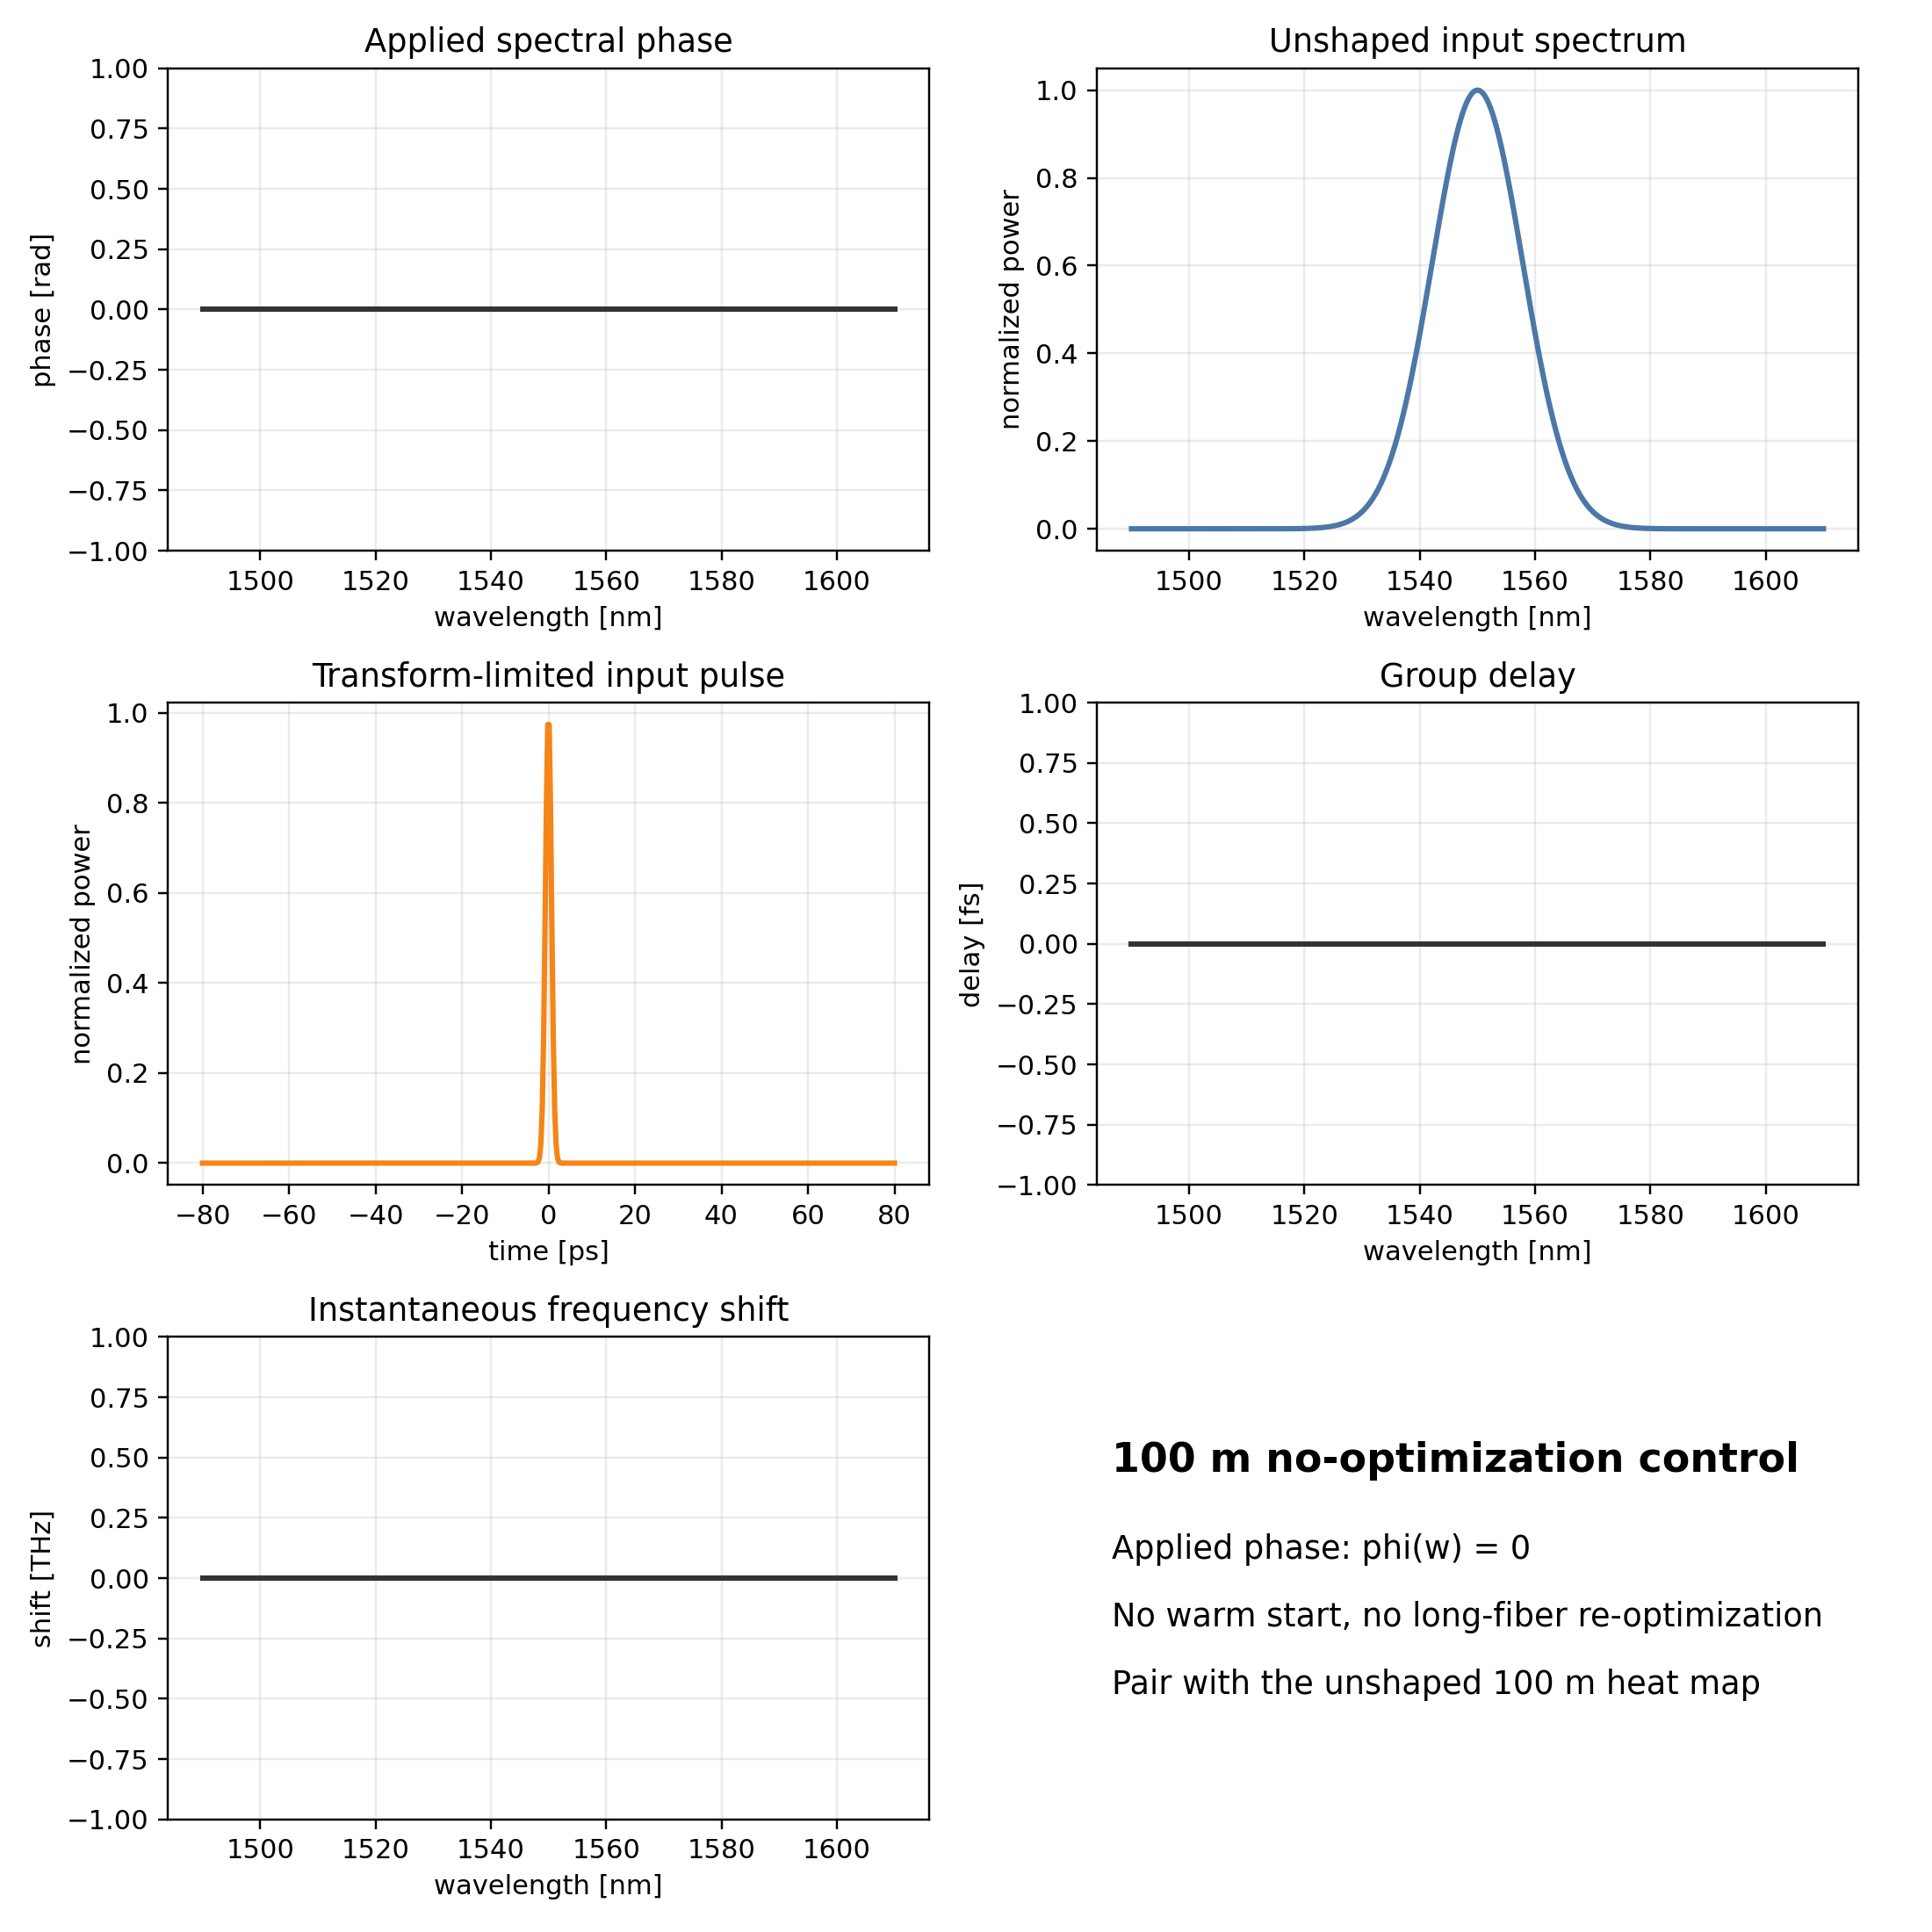
\includegraphics[height=0.47\textheight]{figures/longfiber100m_no_optimization_phase_diagnostic.png}
\vspace{0.5em}

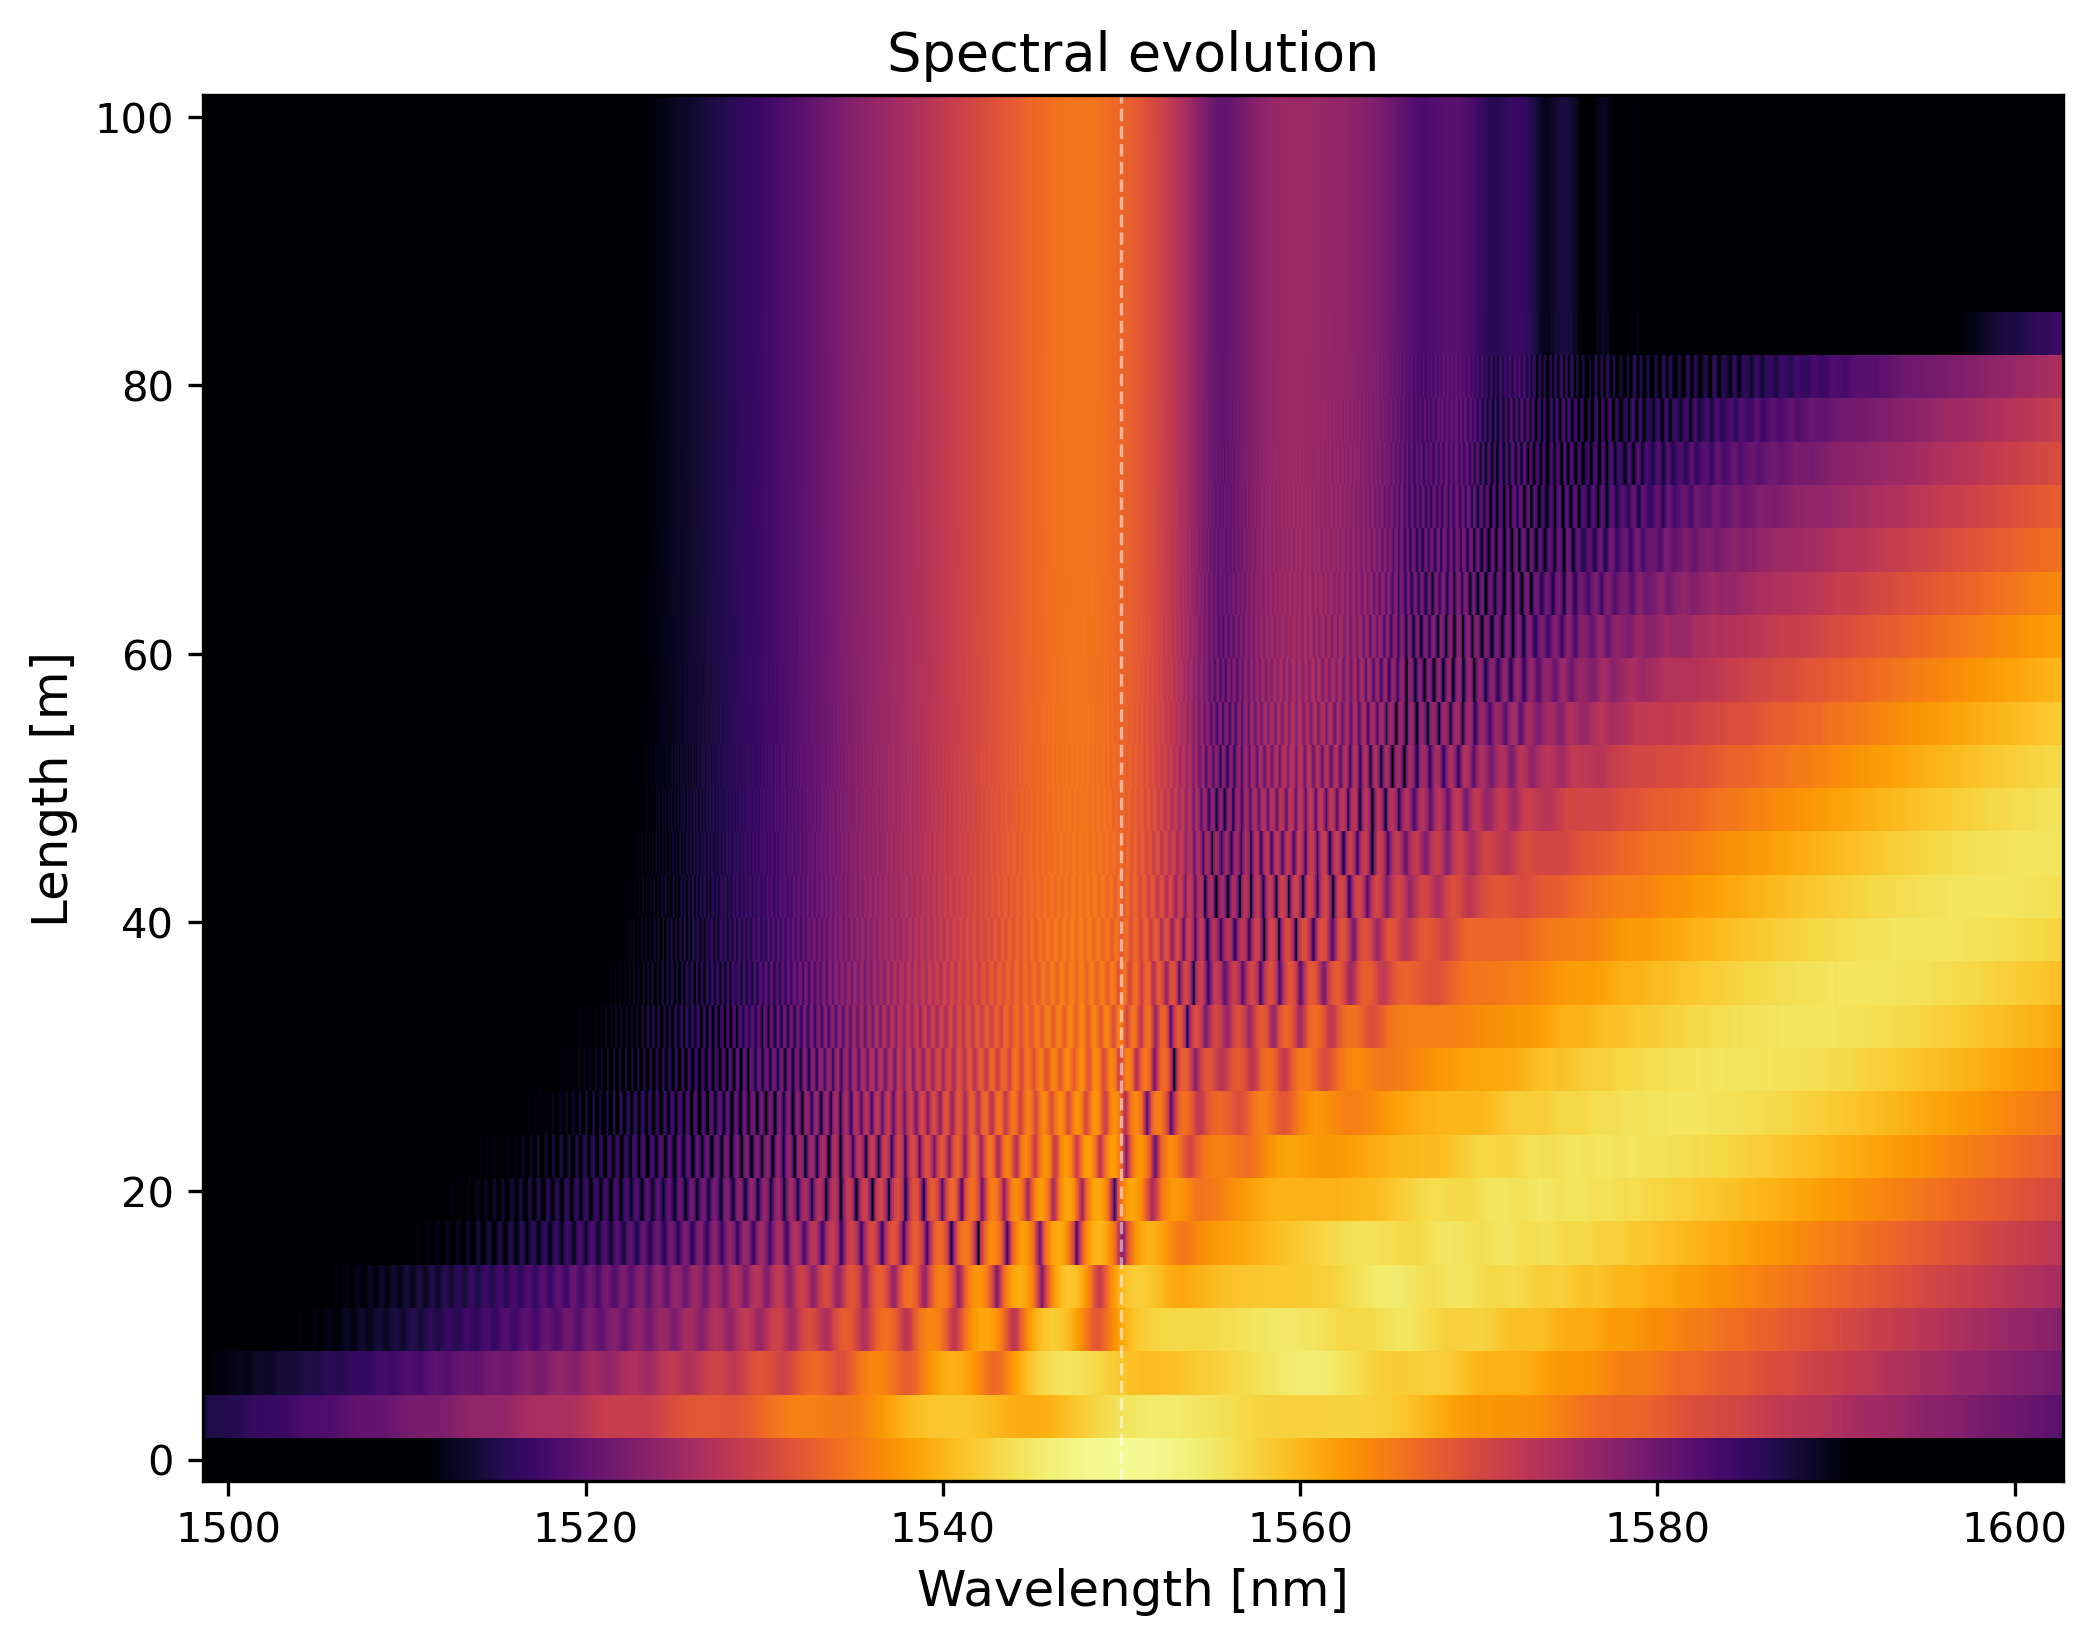
\includegraphics[height=0.31\textheight]{figures/longfiber100m_unshaped_evolution.png}
\caption{No-shaping control for the $100$ m long-fiber setting.  The phase
diagnostic shows that no spectral phase was applied; the heat map is the
reference case for judging whether the optimized and warm-started masks are
doing real Raman suppression rather than only changing the plotted scale.}
\label{fig:control}
\end{figure}

\clearpage
\section{Optimized Long-Fiber Example}

\begin{figure}[H]
\centering
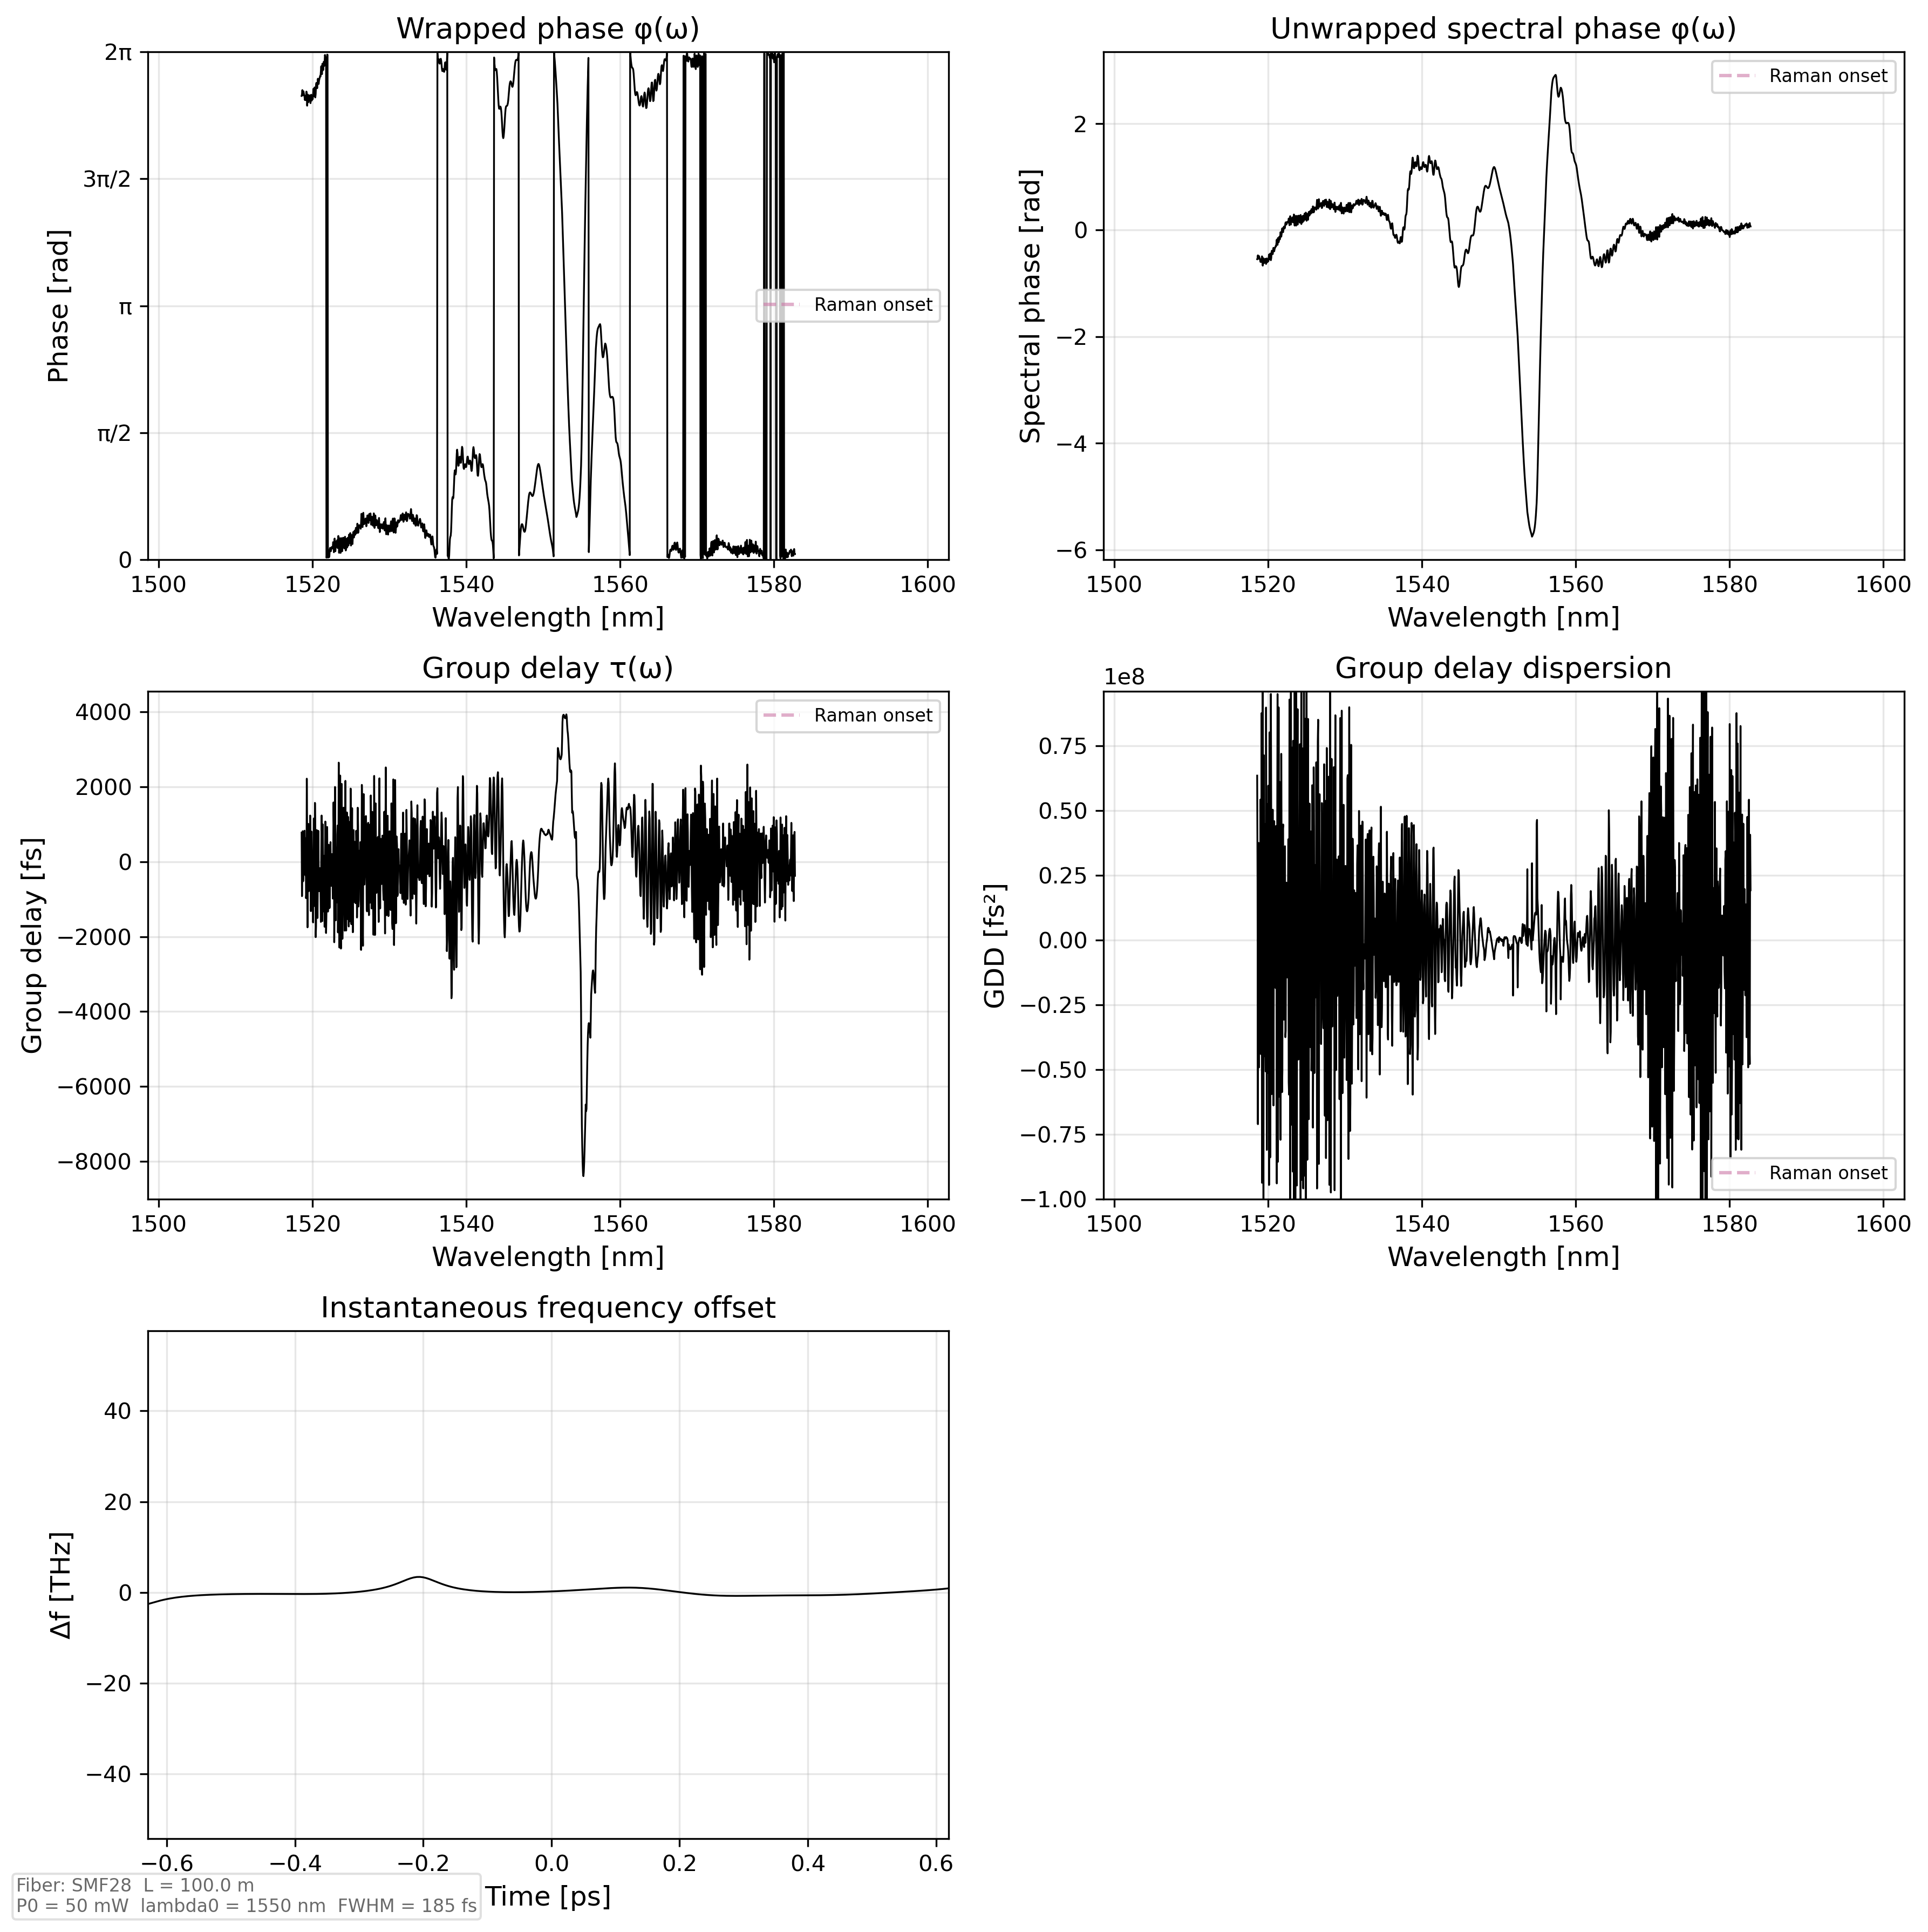
\includegraphics[height=0.47\textheight]{figures/longfiber100m_reoptimized_phase_diagnostic.png}
\vspace{0.5em}

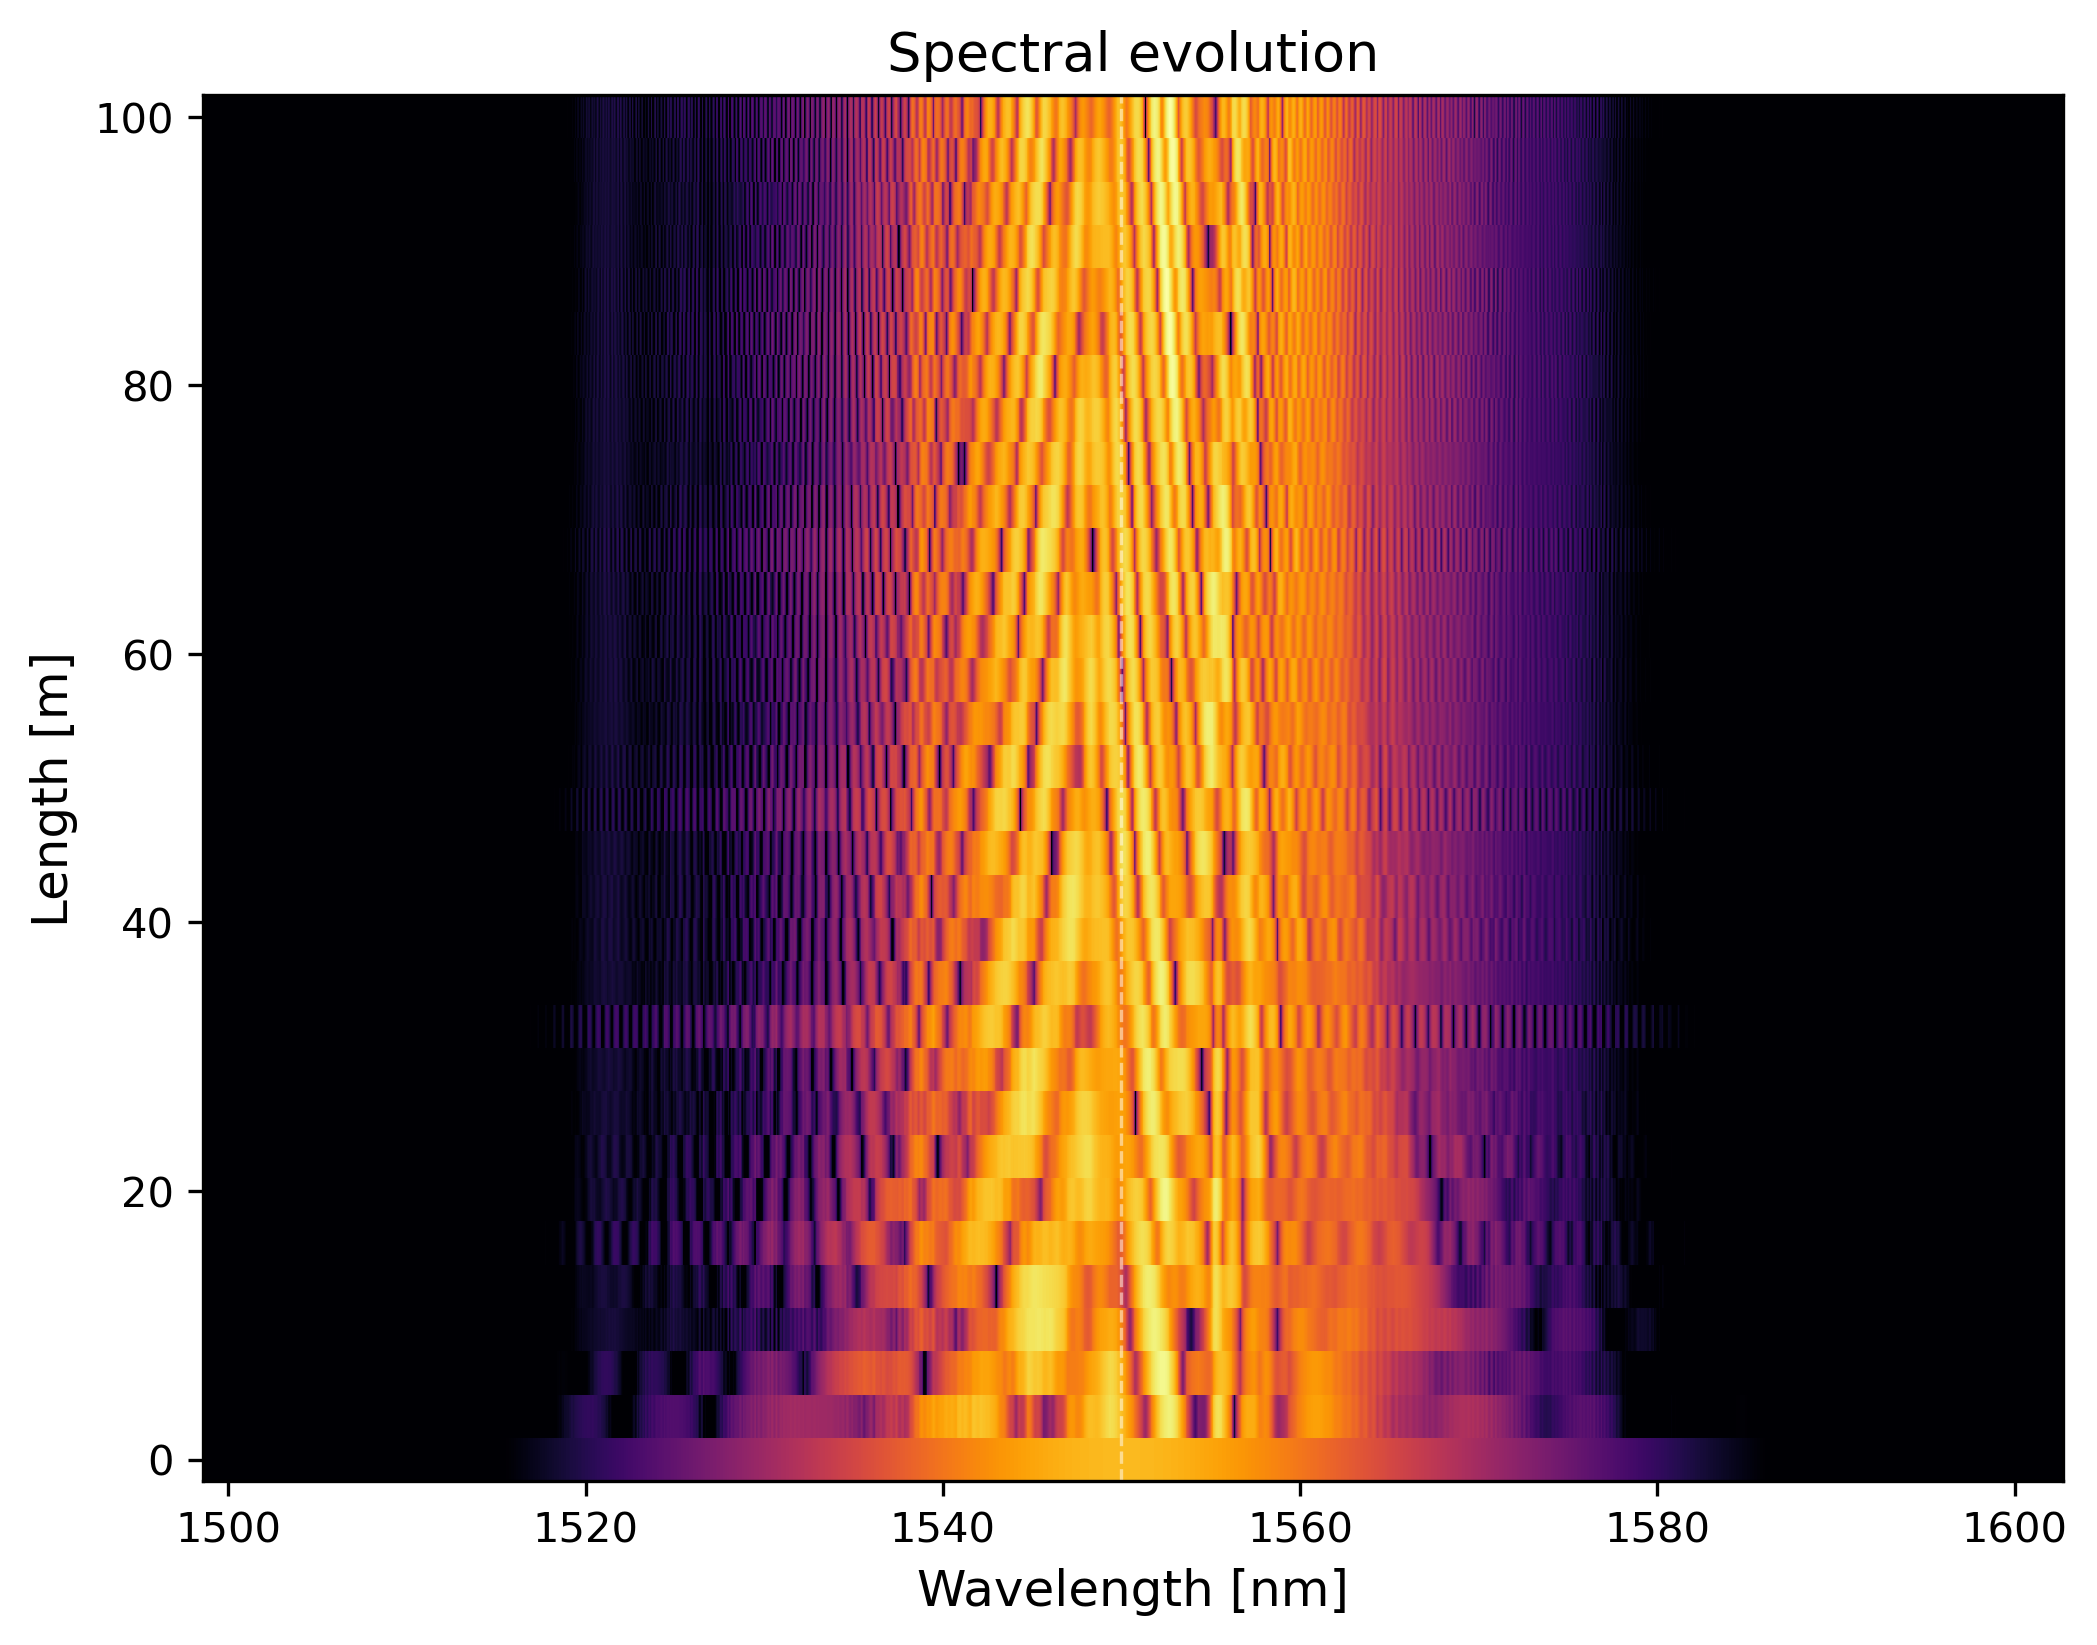
\includegraphics[height=0.31\textheight]{figures/longfiber100m_reoptimized_evolution.png}
\caption{Warm-start re-optimized $100$ m example.  The diagnostic is useful,
but the profile is visibly rough; this is why the result is presented as a
compute-strategy result rather than a lab-ready waveform prescription.  The
matching heat map is the main visual evidence that the phase mask changes the
Raman transfer path.}
\label{fig:optimized-pair}
\end{figure}

\section{Interpretation}

The result suggests a useful split between \emph{basin finding} and
\emph{basin refinement}.  The short-fiber mask appears to contain much of the
structure needed to avoid Raman transfer even over much longer propagation.
The long-fiber re-optimization then adjusts that structure for the specific
long target.

The long-fiber phase is not safely described as ``just a quadratic chirp.''
The recorded quadratic-fit checks found poor polynomial fit quality over the
amplitude-weighted pulse band, and pure dispersion-length scaling did not
predict the long-fiber phase coefficient.  That matters because it means the
warm start is carrying nonlinear structural information, not only a simple GVD
pre-compensation.

\paragraph{TL;DR.}
The short mask is not magic, and it is not guaranteed to be the final answer.
It is a strong first guess.  For expensive long fibers, that may be the
difference between a tractable optimization and a blind search.

\section{Presentation Capsule}

If this note becomes a long-fiber strategy slide, the clean message is:
\begin{itemize}
\item Long-fiber optimization is expensive, so initialization matters.
\item A short-fiber optimized mask can act as a warm start for the long target, then the optimizer adapts it to the longer propagation length.
\item The visual story should be the $100$ m no-shaping control versus the optimized long-fiber heat map, not an internal run-history label.
\item The result is a practical strategy note, not proof of a globally optimal $100$ m waveform.
\end{itemize}

\section{Limitations}

\begin{itemize}
\item The $100$ m re-optimized runs did not satisfy a strict convergence claim;
the final gradient norms remain too large to call this a completed optimum.
\item The evidence is single-mode.  Multimode long-fiber optimization should
not inherit these results automatically.
\item The current note does not prove that warm-starting is cheaper than every
possible cold-start strategy; it shows that the warm start reaches a very good
basin and gives a practical compute path.
\item A real segmented hardware experiment would need in-line shaping or some
other way to modify the field after partial propagation.  The current workflow
only changes the numerical optimizer initialization.
\item The $100$ m phase diagnostic is rough.  That is acceptable for a research
strategy note, but not for a final lab waveform prescription.
\end{itemize}

\section{Reproduction Capsule}

For a clean reproduction, run on the heavy-compute machine with Julia threading
enabled.  The relevant public workflow surface is in
\texttt{scripts/research/longfiber/}:
\begin{itemize}
\item \texttt{longfiber\_setup.jl}: constructs the long-fiber problem while
honoring the requested grid and time window.
\item \texttt{longfiber\_optimize\_100m.jl}: runs the warm-started long-fiber
L-BFGS optimization.
\item \texttt{longfiber\_validate\_100m.jl}: checks the final result and
reports the evidence numbers.
\item \texttt{longfiber\_regenerate\_standard\_images.jl}: regenerates the
standard diagnostic image set when needed.
\end{itemize}

The required output artifacts are the final cost, convergence flag, gradient
norm, energy drift, boundary/edge fraction, and the standard image set:
phase profile, phase diagnostic, optimized evolution, and unshaped evolution.
The note should not be upgraded from provisional to production-ready until a
fresh rerun confirms these artifacts and the PDF figures are visually checked
again.

\section{Sources}

\begin{itemize}
\item G. P. Agrawal, \emph{Nonlinear Fiber Optics}, 6th ed., Academic Press,
2019.  Standard reference for the generalized nonlinear Schr\"odinger model,
Kerr nonlinearity, dispersion, and stimulated Raman scattering.
\item J. Hult, ``A fourth-order Runge--Kutta in the interaction picture method
for simulating supercontinuum generation in optical fibers,'' \emph{Journal of
Lightwave Technology}, 25(12), 3770--3775, 2007.
\url{https://doi.org/10.1109/JLT.2007.909373}
\item J. Nocedal and S. J. Wright, \emph{Numerical Optimization}, 2nd ed.,
Springer, 2006.  Reference for L-BFGS, line-search methods, and convergence
diagnostics. \url{https://doi.org/10.1007/978-0-387-40065-5}
\item E. L. Allgower and K. Georg, \emph{Numerical Continuation Methods},
Springer, 1990.  Reference background for continuation-style warm starts.
\url{https://doi.org/10.1007/978-3-642-61257-2}
\end{itemize}

\end{document}
